\documentclass[a4paper]{article}
\usepackage[14pt]{extsizes}
\usepackage[utf8]{inputenc}
\usepackage[russian]{babel}
\usepackage{setspace,amsmath}
\usepackage{graphicx}
\usepackage{hyperref}
\usepackage[left=20mm, top=15mm, right=15mm, bottom=15mm, nohead, footskip=10mm]{geometry} % настройки полей документа
\graphicspath{./image/}
\usepackage{graphics}

\begin{document} % начало документа

% НАЧАЛО ТИТУЛЬНОГО ЛИСТА
\begin{center}
\hfill \break
\large{МИНИСТЕРСТВО НАУКИ И ВЫСШЕГО ОБРАЗОВАНИЯ РОССИЙСКОЙ ФЕДЕРАЦИИ}\\
\footnotesize{федеральное государственное автономное образовательное учреждение высшего образования}\\
\small{\textbf{«САНКТ-ПЕТЕРБУРГСКИЙ ГОСУДАРСТВЕННЫЙ УНИВЕРСИТЕТ АЭРОКОСМИЧЕСКОГО ПРИБОРОСТРОЕНИЯ»}}\\
\hfill \break
\normalsize{КАФЕДРА №25}\\
\hfill \break
\hfill\break
\hfill\break
\hfill \break
\hfill \break
\hfill \break
\large{Сервлет с анекдотами}\\
\hfill \break
\hfill \break
\hfill \break
\normalsize{Функциональная спецификация к курсовой работе\\
\hfill \break
по курсу: ТЕХНОЛОГИИ ПРОГРАММИРОВАНИЯ\\
\hfill \break
\hfill \break
\hfill \break
\end{center}
\hfill \break
\normalsize{

\begin{tabular}{cccc}
Преподаватель:\\\\
Доцент, к.т.н. & \underline{\hspace{6cm}} & Е. М. Линский \\\\
Работу выполнил:\\\\
Студент гр. №2051 & \underline{\hspace{6cm}} & Э. С. Чуриков \\\\
\end{tabular}
}\\
\hfill \break
\hfill \break
\begin{center} Санкт-Петербург 2022 \end{center}
\thispagestyle{empty} % выключаем отображение номера для этой страницы
% КОНЕЦ ТИТУЛЬНОГО ЛИСТА

\clearpage
\section{Постановка задачи}
Сервлет с анекдотами
\begin{itemize}
\item На сервере хранятся списком анекдоты в текстовом файле.
\item В ответ на запрос клиента сервер присылает из этого списка случайный анекдот.

\end{itemize}

\section{Архитектура}
На оценку 3:
\begin{itemize}
\item проект должен запускаться из командной строки

\end{itemize}


\section{Функционал пользователя}
\begin{itemize}
\item Установка соединения с сервером и получение анекдота.
\item Нажатие на кнопку "получить анекдот" для обновления анекдота.

\end{itemize}


\section{Пример программы}
\begin{center}
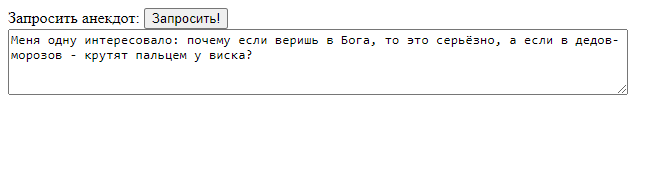
\includegraphics[scale = 0.6]{humor1.png}

Рисунок 1. Пример анекдота при подключении

\hfill \break
\hfill \break
\hfill \break

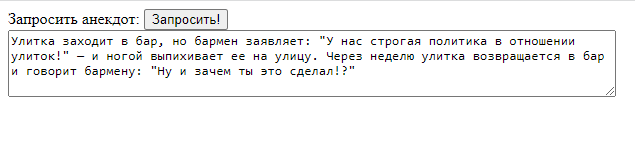
\includegraphics[scale = 0.9]{humor2.png}

Рисунок 2. Пример анекдота при нажатии кнопки "Получить!"
\end{center}
\end{document}